%!TEX program=xelatex

\documentclass[12pt,a4paper,UTF8]{article}
\usepackage[fontset=fandol]{ctex} % Chinese support, using Fandol fonts
\usepackage{graphicx} % Insert images
\usepackage{listings} % Print source code
\usepackage{color} % Color support
\usepackage{booktabs} % Professional table support
\usepackage{pdflscape} % Landscape pages support in PDF
\usepackage{hyperref} % Hypertext links support for cross-referencing
\usepackage{background}

% Customize hyperref format (it's set to no special format here)
\hypersetup{hidelinks}

% Declare directories to search for graphics files for graphicx
\graphicspath{{figures/}{logo/}}

% 自定义代码块样式
\lstset
{
    language=C++,
    basicstyle=\ttfamily\footnotesize,
    keywordstyle=\bfseries\color[rgb]{0, 0, 1},
    identifierstyle=\color[rgb]{0.5, 0.3, 0.1},
    stringstyle=\color[rgb]{0.6, 0.1, 0.1},
    commentstyle=\itshape\color[rgb]{0.05, 0.5, 0.05},
    backgroundcolor=\color[gray]{0.95},
    numbers=left,
    numbersep=5pt,
    numberstyle=\color[gray]{0.6},
    breaklines=true
} 

% Define source code style for listings
\lstdefinestyle{cpp-style}{
    language=C++,
    basicstyle=\ttfamily\footnotesize,
    keywordstyle=\bfseries\color[rgb]{0, 0, 1},
    identifierstyle=\color[rgb]{0.5, 0.3, 0.1},
    stringstyle=\color[rgb]{0.6, 0.1, 0.1},
    commentstyle=\itshape\color[rgb]{0.05, 0.5, 0.05},
    backgroundcolor=\color[gray]{0.95},
    numbers=left,
    numbersep=5pt,
    numberstyle=\color[gray]{0.6},
    breaklines=true
}

% Define new command for title page
\newcommand{\reporttitle}[2]{
    \LARGE\textsf{#1}\quad\underline{\makebox[12em]{#2}}
}
\newcommand{\reportinfo}[2]{
    \large\makebox[4em]{\textsf{#1}}\quad\underline{\makebox[18em]{#2}}
}

% The document begins here
\begin{document}
    %Background settings
    \backgroundsetup{scale=2,angle=0,opacity=0.5,pages='some',contents={
\includegraphics[width=\paperwidth,height=\paperwidth,keepaspectratio]{pictures/background.png}}}

    \begin{titlepage}
        \centering
        \vspace*{\fill}    
        \BgThispage
        {\huge\textsf{实\ 验\ 报\ 告}}\\[48pt]
        \reporttitle{实验名称}{Latex实验报告设计}\\[8pt]
        \reporttitle{}{和git版本控制}\\[72pt]
        \reportinfo{课程名称}{系统开发工具基础}\\[8pt]
        \reportinfo{学\hspace{\fill}号}{23070001092}\\[8pt]
        \reportinfo{学生姓名}{王佳晖}\\[8pt]
        \reportinfo{实验日期}{2024年8月23日}\\
        \vspace*{\fill}
    \end{titlepage}

    \tableofcontents
    \newpage

    \NoBgThispage
    \section{实验目的}
    \begin{enumerate}    
        \item 学习Latex文档编辑的使用方法
        \item 学习使用git进行版本控制
    \end{enumerate}
    
    \section{实验内容}
    \subsection{使用Latex制作个人模版}
    \begin{enumerate}
        \item \textcolor{blue}{usepackage语句:用于引用Latex宏包}\\
        样例:\textbackslash usepackage\{color\}\\[8pt]
        部分常见的宏包名称和作用如下,详见表 \ref{broomsticks}
        \begin{table}[htbp]
            \centering
            \begin{tabular}{cccc}
                \toprule
                序号 & 名称 & 作用 \\
                \midrule
                1 & \textcolor{red}{graphicx} & 插入和调整图片。 \\
                2 & \textcolor{red}{booktabs} & 创建更美观的表格线和表格布局。 \\
                3 & \textcolor{red}{hyperref} & 创建可点击的链接、书签和引用。 \\
                4 & \textcolor{red}{listings} & 插入和调整代码。 \\
                \bottomrule
            \end{tabular}
            \caption{部分常见的宏包}
            \label{broomsticks}
        \end{table}
        
        \item \textcolor{blue}{textcolor语句:用于修改文字颜色}\\
        样例:\textbackslash textcolor\{red\}\{红色\}\\
        效果:
\includegraphics{pictures/Latex/2.png}

        \item \textcolor{blue}{includegraphics语句:用于显示图片}\\
        样例:\textbackslash includergraphics[width=20,height=10]\{2.png\}\\
        效果:\\
        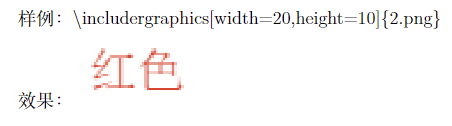
\includegraphics[scale=0.75]{pictures/Latex/3.png}

        
        \item \textcolor{blue}{begin和end语句:是用于定义和包围环境}\\[8pt]
        注:环境是LaTeX中的一个核心概念,它们用来指定特定的格式或功能。在环境内,LaTeX会根据环境的类型来决定如何处理和排版内容。\\
        下面是一些常用的环境:

        \item \textcolor{blue}{center环境}\\
        样例:\\
        \textbackslash begin\{center\}\\
        中间这段文字将要居中显示\\
        \textbackslash end\{center\}\\
        效果:\\
        \begin{center}
            中间这段文字将要居中显示
        \end{center}
        \bigskip
        
        \item \textcolor{blue}{equation环境:}\\
        样例:\\
        \textbackslash begin\{equation\}\\
        E=mc\textasciicircum2\\
        \textbackslash end\{equationr\}\\
        效果:\\
        \begin{equation}
            E=mc^2
        \end{equation}
        \bigskip

        \item \textcolor{blue}{lstlisting环境:}\\
        样例:\\
        \textbackslash begin\{lstlisting\}[language=C++]\\
        \#include<iostream>\\
        using namespace std;\\
        int main()\\
        {\\
            cout<<"HELLO WORLD!";\\
            return 0;\\
        }\\
        \textbackslash end\{lstlisting\}\\
        效果:\\
        \begin{lstlisting}[language=C++]
            #include<iostream>
            using namespace std;
            int main()
            {
                cout<<"HELLO WORLD!";
                return 0;
            }
        \end{lstlisting}
        \bigskip
        
        \item \textcolor{blue}{tabular环境:}\\
        样例:\\
        \textbackslash begin\{tabular\}\{cccc\}\\
            \textbackslash toprule\\
                  \& 第一列 \& 第二列 \& 第三列 \\
            \textbackslash midrule\\
            第一行 \& (1,1) \& (1,2) \& (1,3) \\
            第二行 \& (2,1) \& (2,2) \& (2,3) \\
            第三行 \& (3,1) \& (3,2) \& (3,3) \\
            \textbackslash bottomrule\\
        \textbackslash end\{tabular\}\\
        效果:\\[8pt]
        \begin{tabular}{cccc}
            \toprule
                  & 第一列 & 第二列 & 第三列 \\
            \midrule
            第一行 & (1,1) & (1,2) & (1,3) \\
            第二行 & (2,1) & (2,2) & (2,3) \\
            第三行 & (3,1) & (3,2) & (3,3) \\
            \bottomrule
        \end{tabular}
        \bigskip
        
        \item \textcolor{blue}{章节划分语句}\\
        用法:\\
        LaTeX的章节命令是分级的,通常使用如下顺序:\\
        \textbackslash part\{\}:部分,用于大型文档的分部(如书籍的卷)。\\
        \textbackslash chapter\{\}:章(仅在使用 book 类或类似的文档类时可用)。\\
        \textbackslash section\{\}:一级章节。\\
        \textbackslash subsection\{\}:二级章节。\\
        \textbackslash subsubsection\{\}:三级章节。\\
        \textbackslash paragraph\{\}:段落标题,通常不带编号。\\
        \textbackslash subparagraph\{\}:子段落标题,通常不带编号。\\[8pt]
        样例及效果:\\
        
\includegraphics[scale=0.22]{pictures/Latex/9.png}

        \item \textcolor{blue}{常见特殊符号的输入}\\
        \textbackslash :\textbackslash textbackslash\\
        \textasciicircum:\textbackslash textasciicirum\\
        $\sum$:\$\textbackslash sum\&\\
        \$ :\textbackslash \$\\
        \# :\textbackslash \#\\
        \{ :\textbackslash \{\\
        \} :\textbackslash \}\\
        换行:\textbackslash \textbackslash \\
        
    \end{enumerate}
    

    \NoBgThispage
    \subsection{使用git进行版本控制}
    \begin{enumerate}
        \item \textcolor{blue}{git下载}\\
        进入git官网,下载安装包\\
        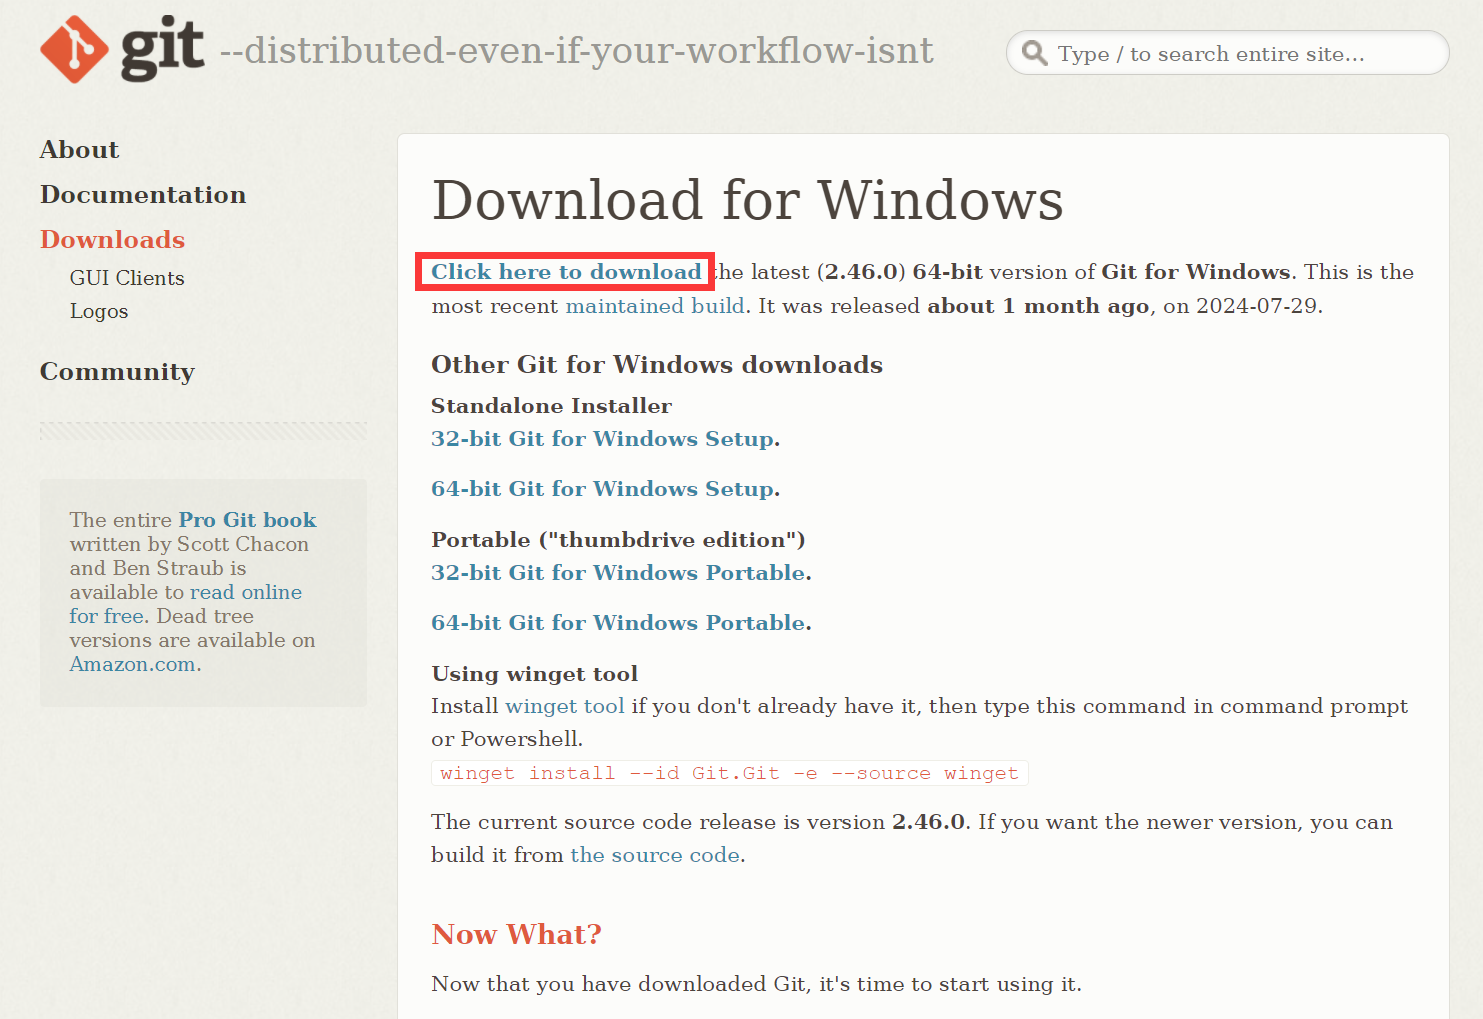
\includegraphics[scale=0.4]{pictures/git/11_1.png}

        \item \textcolor{blue}{git安装}\\
        打开下载好的安装包,按照顺序完成安装选项设置\\
        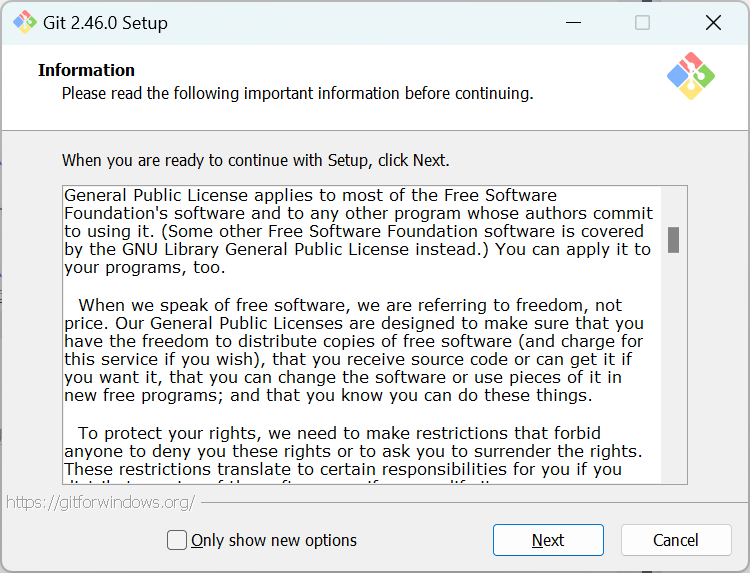
\includegraphics[scale=0.5]{pictures/git/12.png}

        \item \textcolor{blue}{常见git命令}\\[8pt]
        \begin{tabular}{cccc}
            \toprule
            命令        & 作用 \\
            \midrule
            git init   & 创建一个新的 git 仓库,其数据会存放在一个名为 .git 的目录下 \\
            git add    & 添加文件到暂存区 \\
            git commit & 创建一个新的提交 \\
            git push   & 将对象传送至远端并更新远端引用 \\
            git clone  & 克隆远端的库文件 \\
            git log    & 显示历史日志 \\
            git branch & 显示或创建分支 \\
            \bottomrule
        \end{tabular}\\[8pt]

        \textcolor{red}{下面将以本次LaTex个人模版的操作为例,进行git的一系列操作}
        
        \item \textcolor{blue}{cd命令:用于在控制台中切换当前工作目录}\\
        创建一个新文件夹,命名为My LaTex Mould\\
        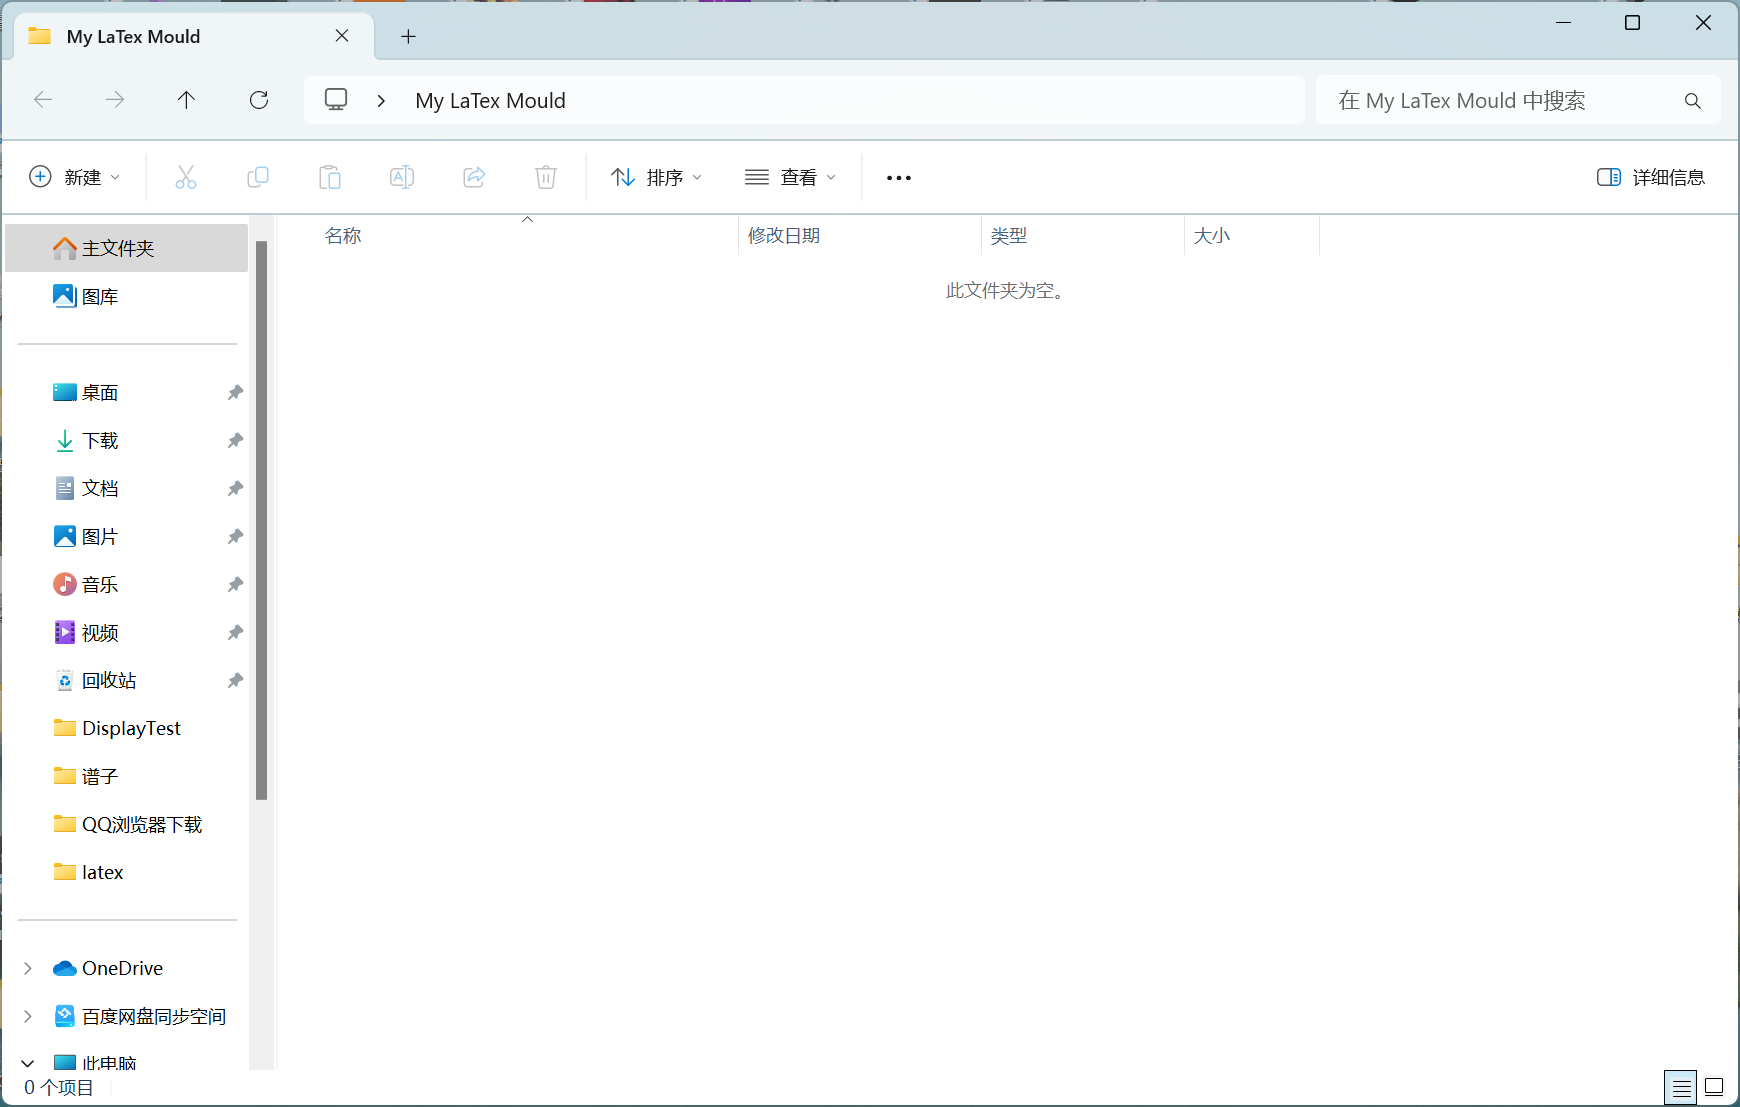
\includegraphics[scale=0.25]{pictures/git/14.png}\\

        打开powershell命令台\\
        使用cd命令,输入刚刚新建文件夹的地址,切换工作目录为此文件夹\\[6pt]
        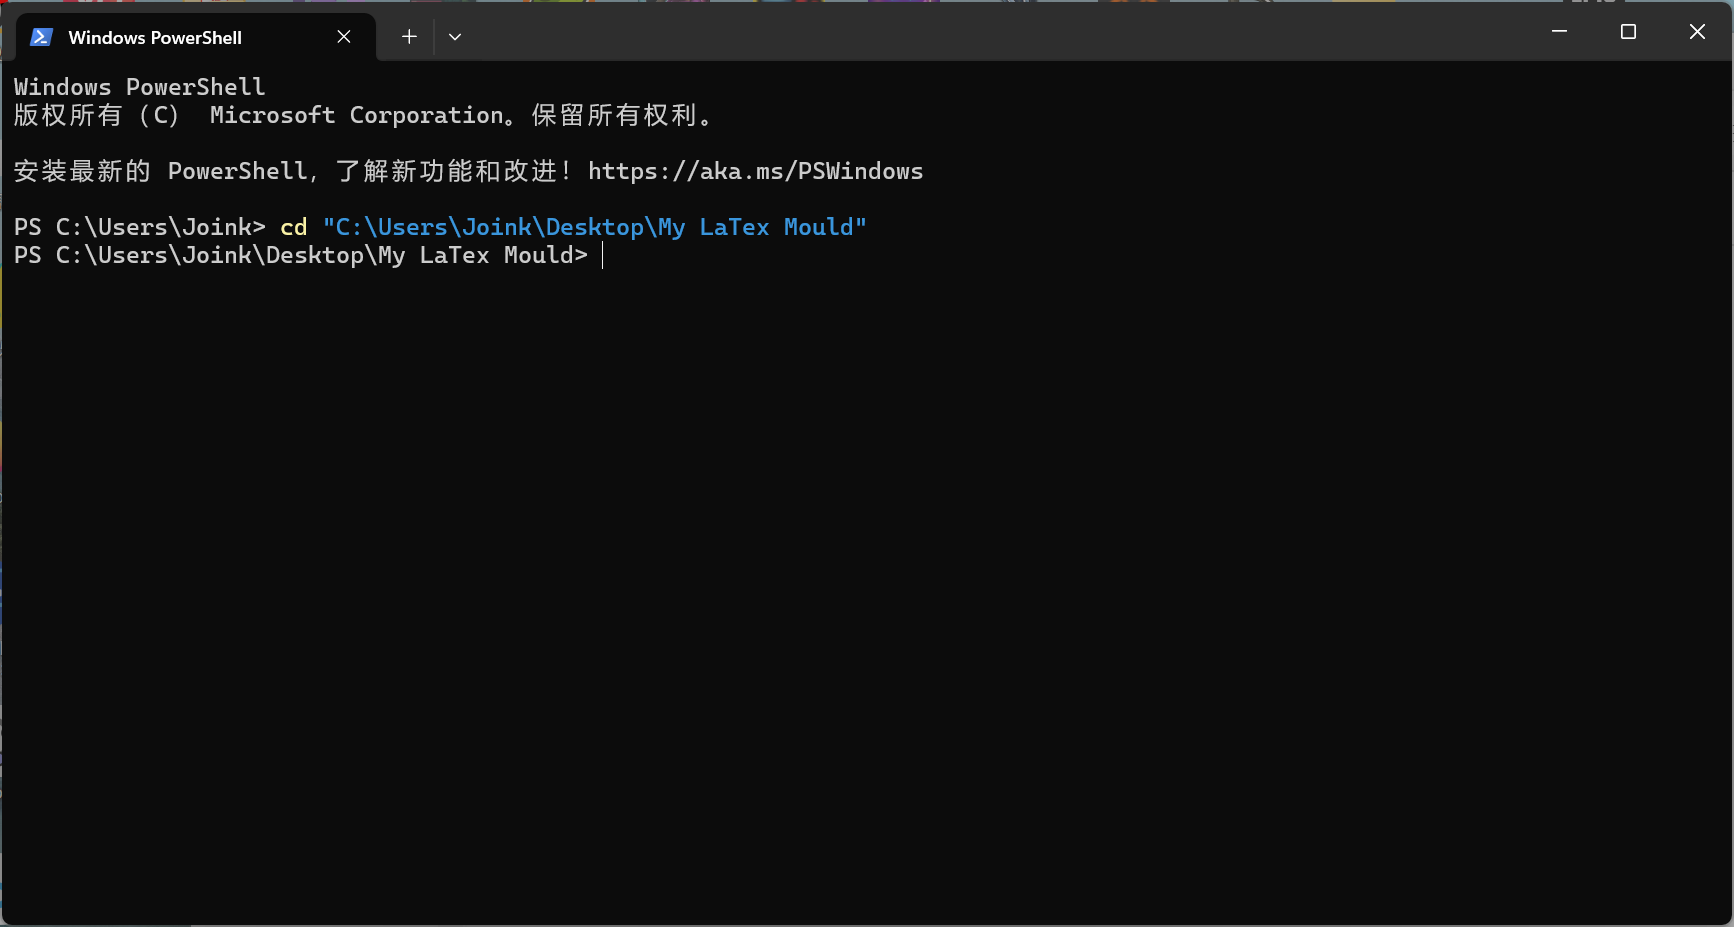
\includegraphics[scale=0.25]{pictures/git/14_2.png}\\
        \textcolor{red}{注:由于文件夹名称中带有空格,而shell命令识别以空格为分界,因此需要给路径加上双引号}

        \item \textcolor{blue}{github项目建立}\\
        打开github网页,点击New respository\\[6pt]
        
\includegraphics[scale=0.25]{pictures/git/15_1.png}\\
        填写好新建项目信息\\[6pt]
        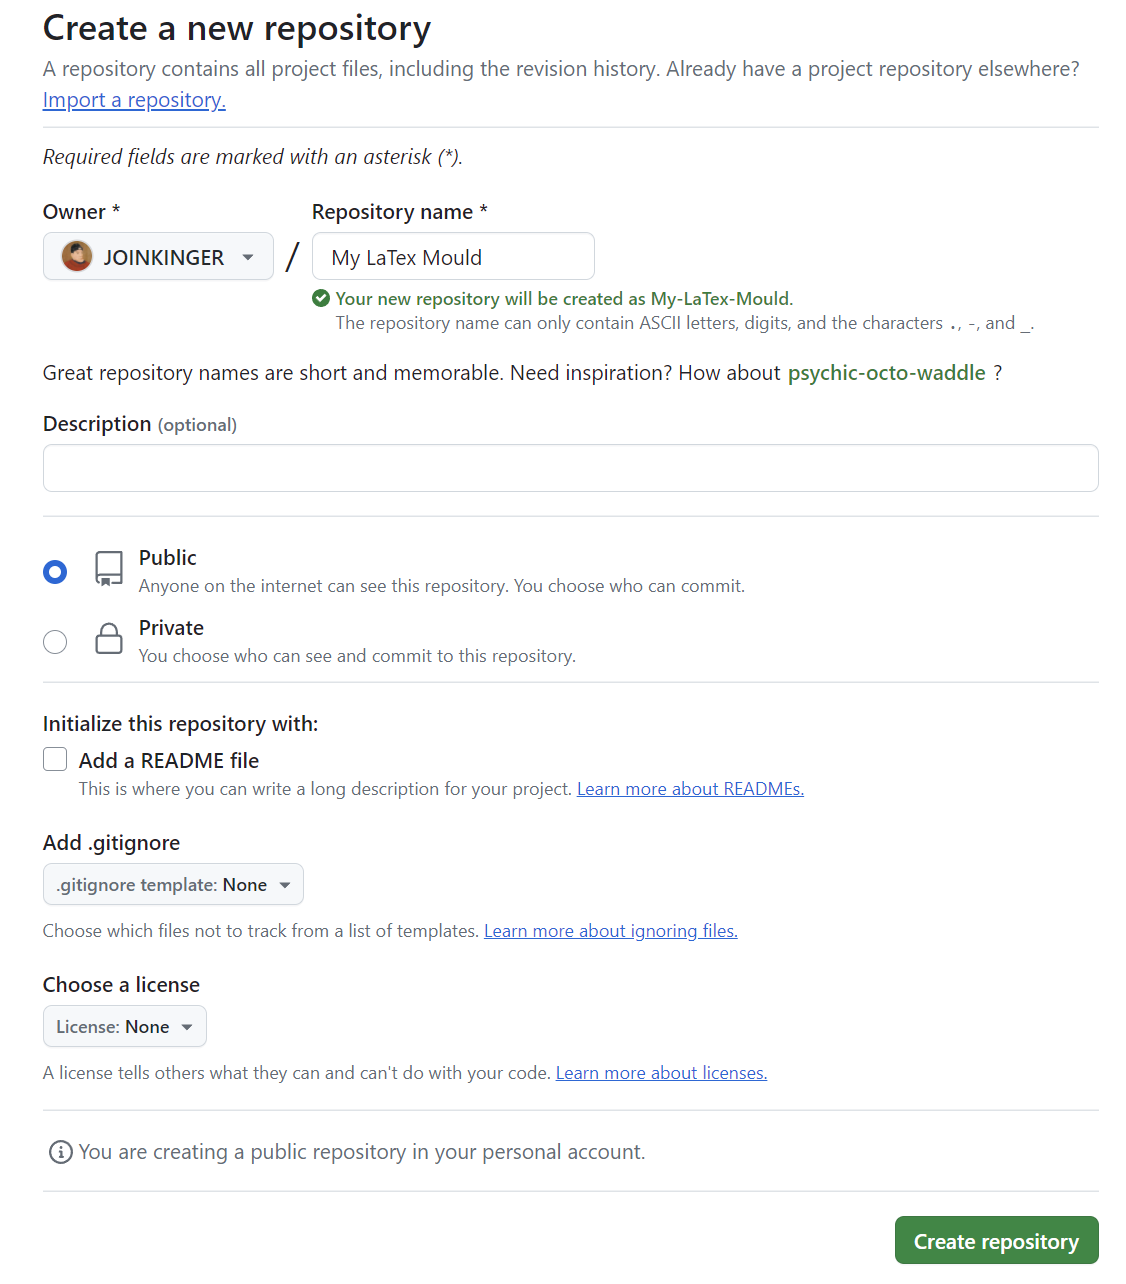
\includegraphics[scale=0.25]{pictures/git/15_2.png}\\
        复制库网址\\[6pt]
        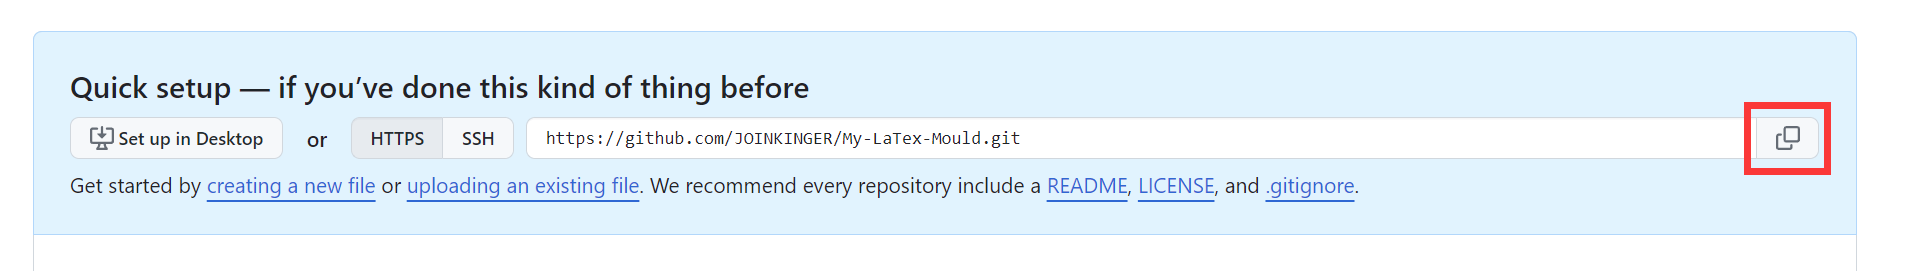
\includegraphics[scale=0.25]{pictures/git/15_3.png}\\
        
        \item \textcolor{blue}{git clone命令}\\
        回到powershell中\\
        使用git clone命令,将刚才github上新建的库clone下来\\[6pt]
        \textcolor{red}{注:这么做的目的是为了后续方便上传到github中}\\
        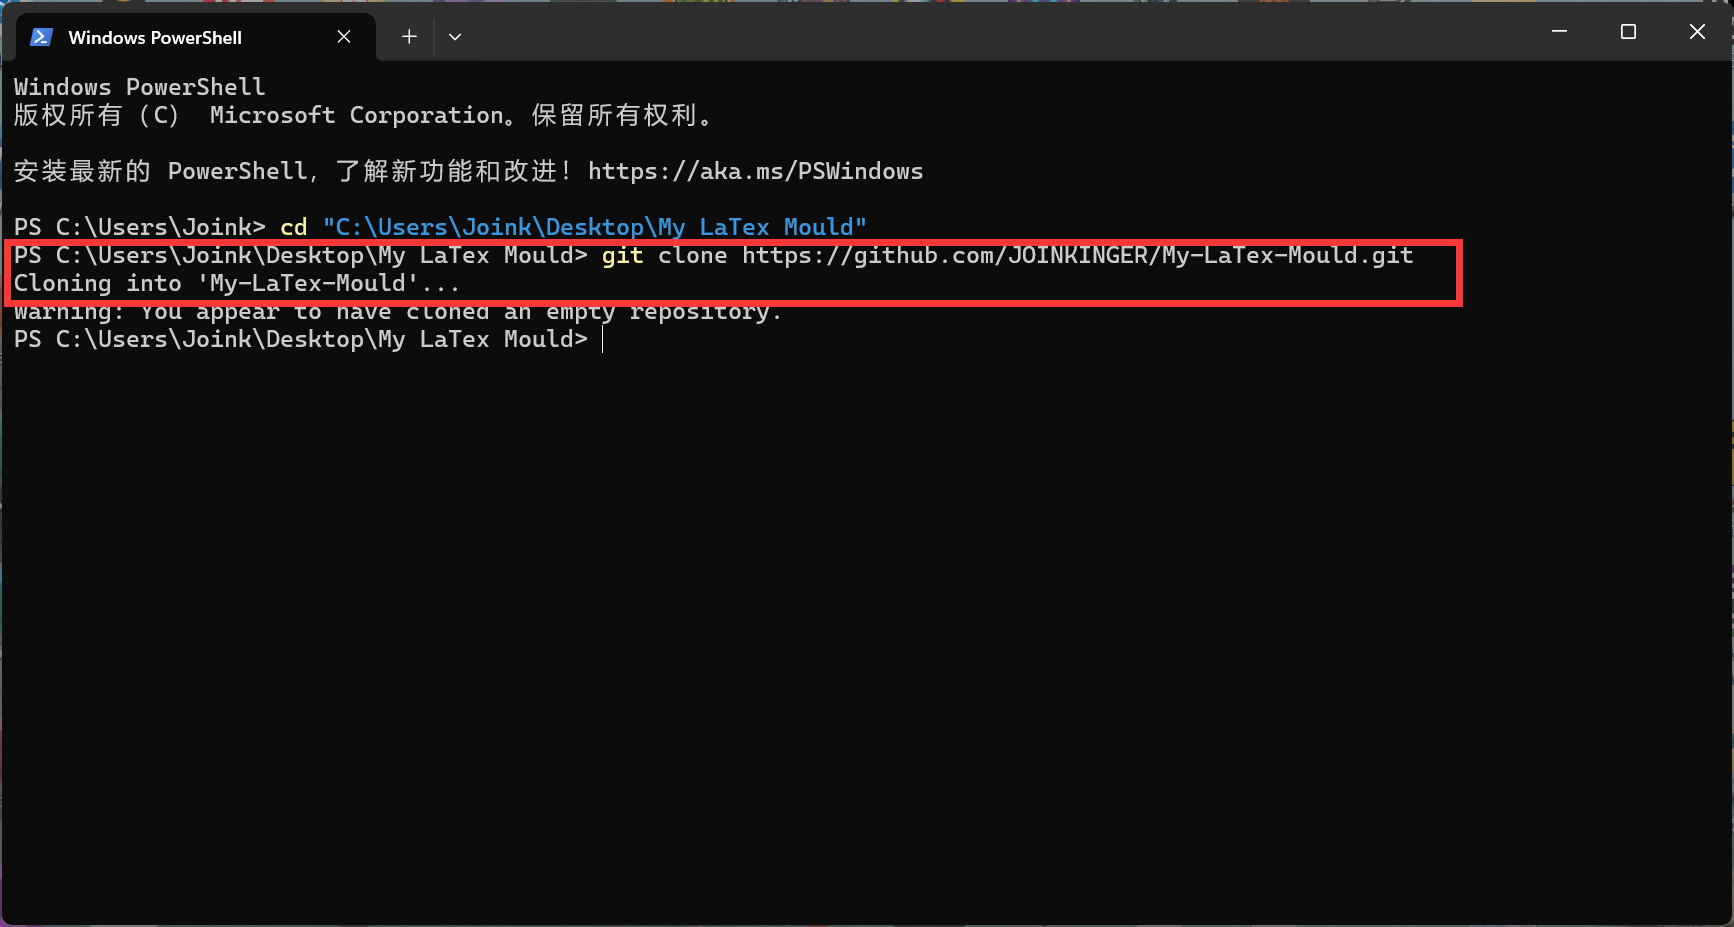
\includegraphics[scale=0.25]{pictures/git/16.png}
        此处警告可以忽视
        
        \item \textcolor{blue}{git add命令}\\
        在overleaf上将LaTex文件保存到本地,拷贝至之前clone下来的文件夹中\\[6pt]
        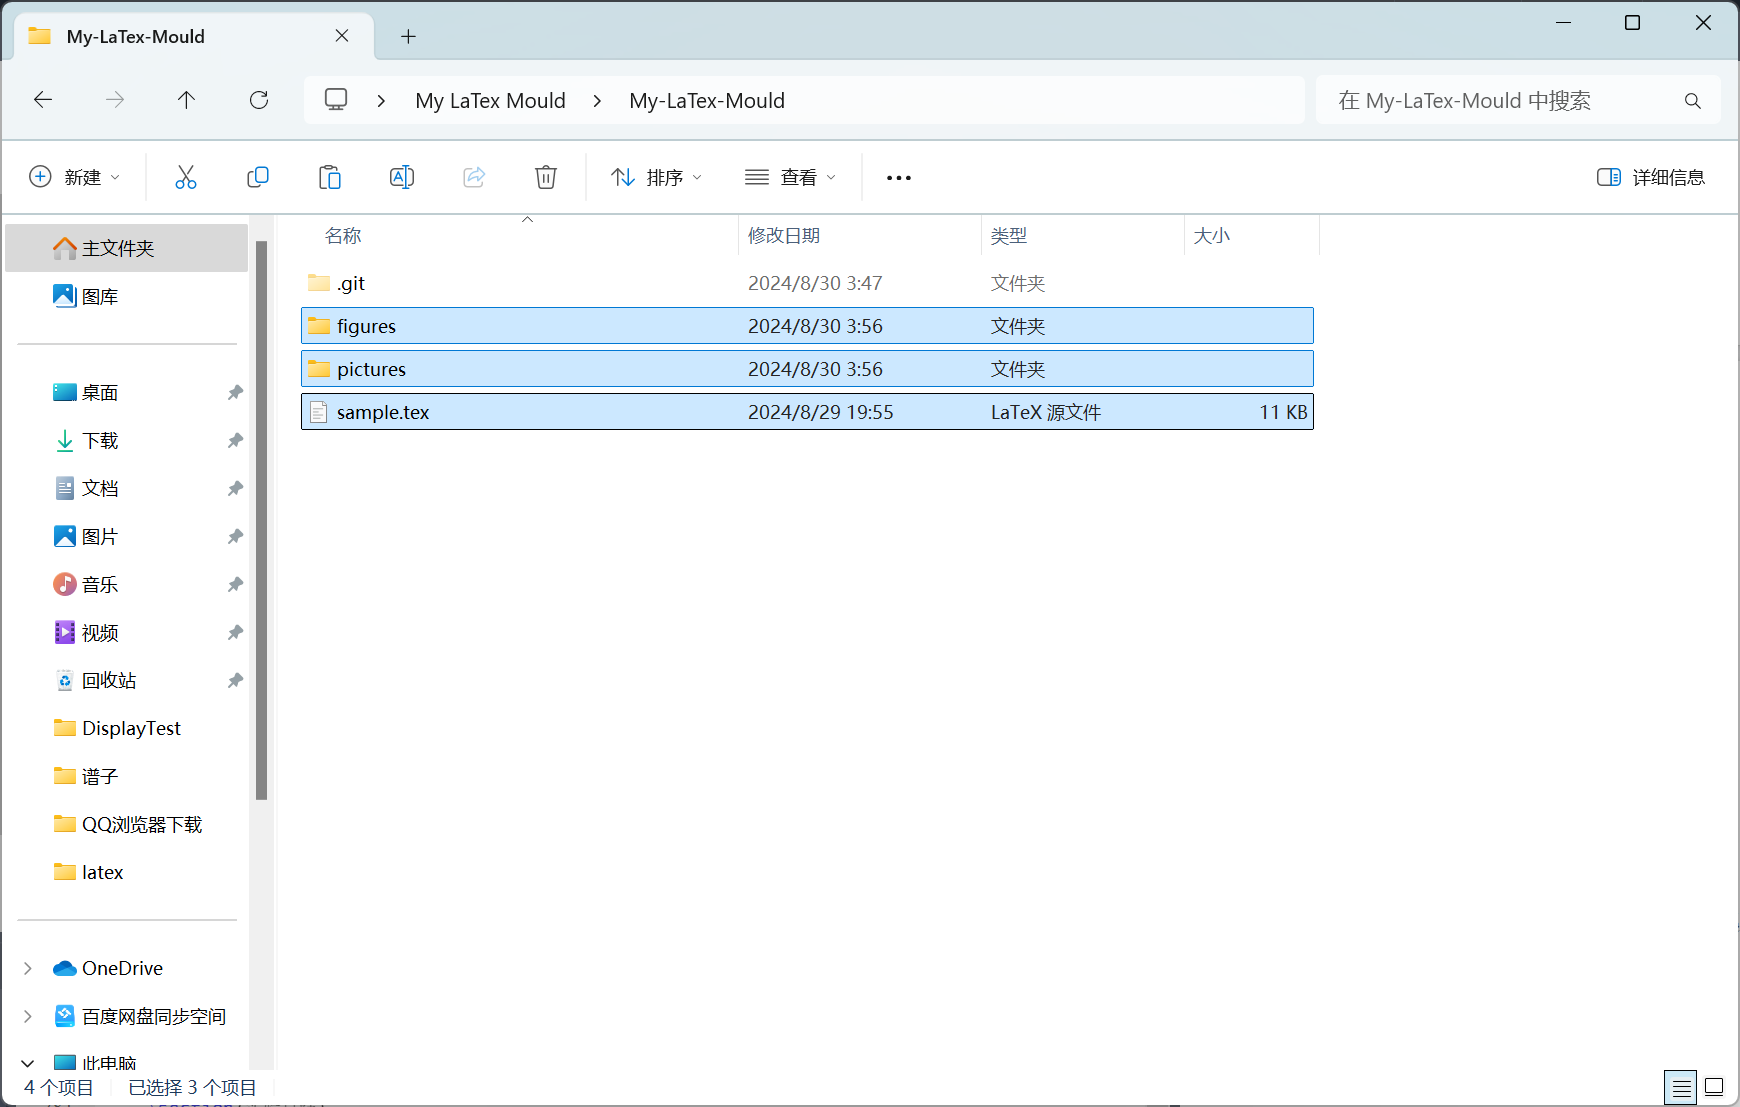
\includegraphics[scale=0.25]{pictures/git/17.png}\\
        回到powershell中\\
        使用cd命令,切换工作目录到clone文件夹\\[6pt]
        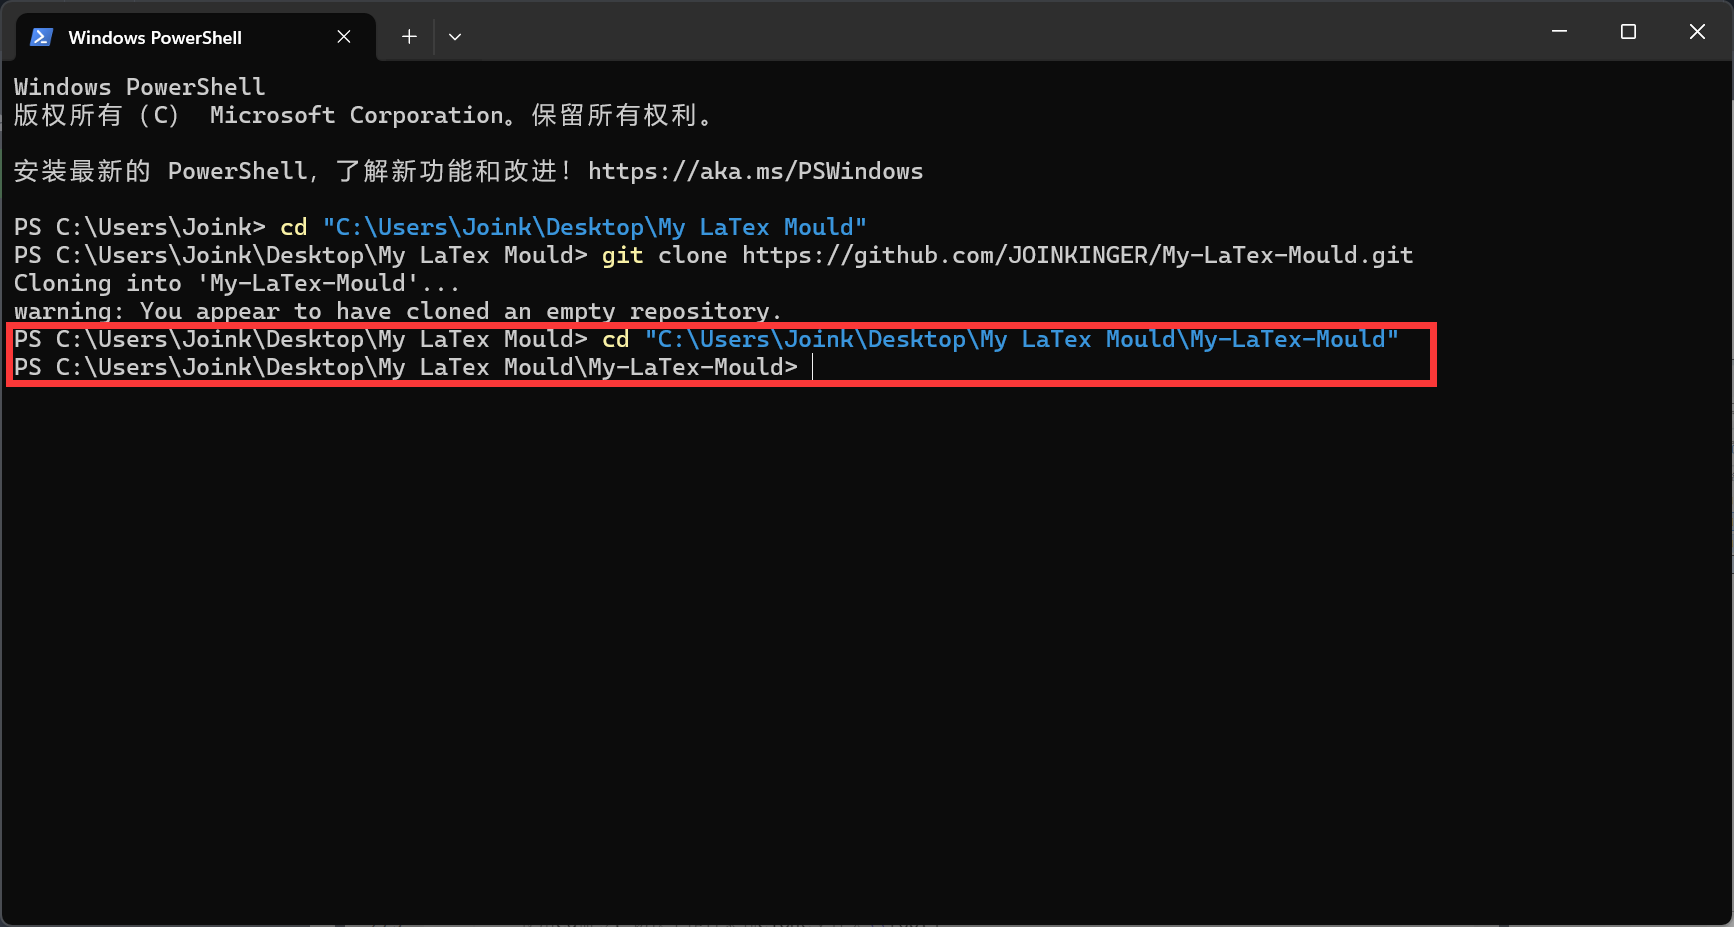
\includegraphics[scale=0.25]{pictures/git/17_2.png}\\
        使用git add命令,添加这些文件到暂存区\\[6pt]
        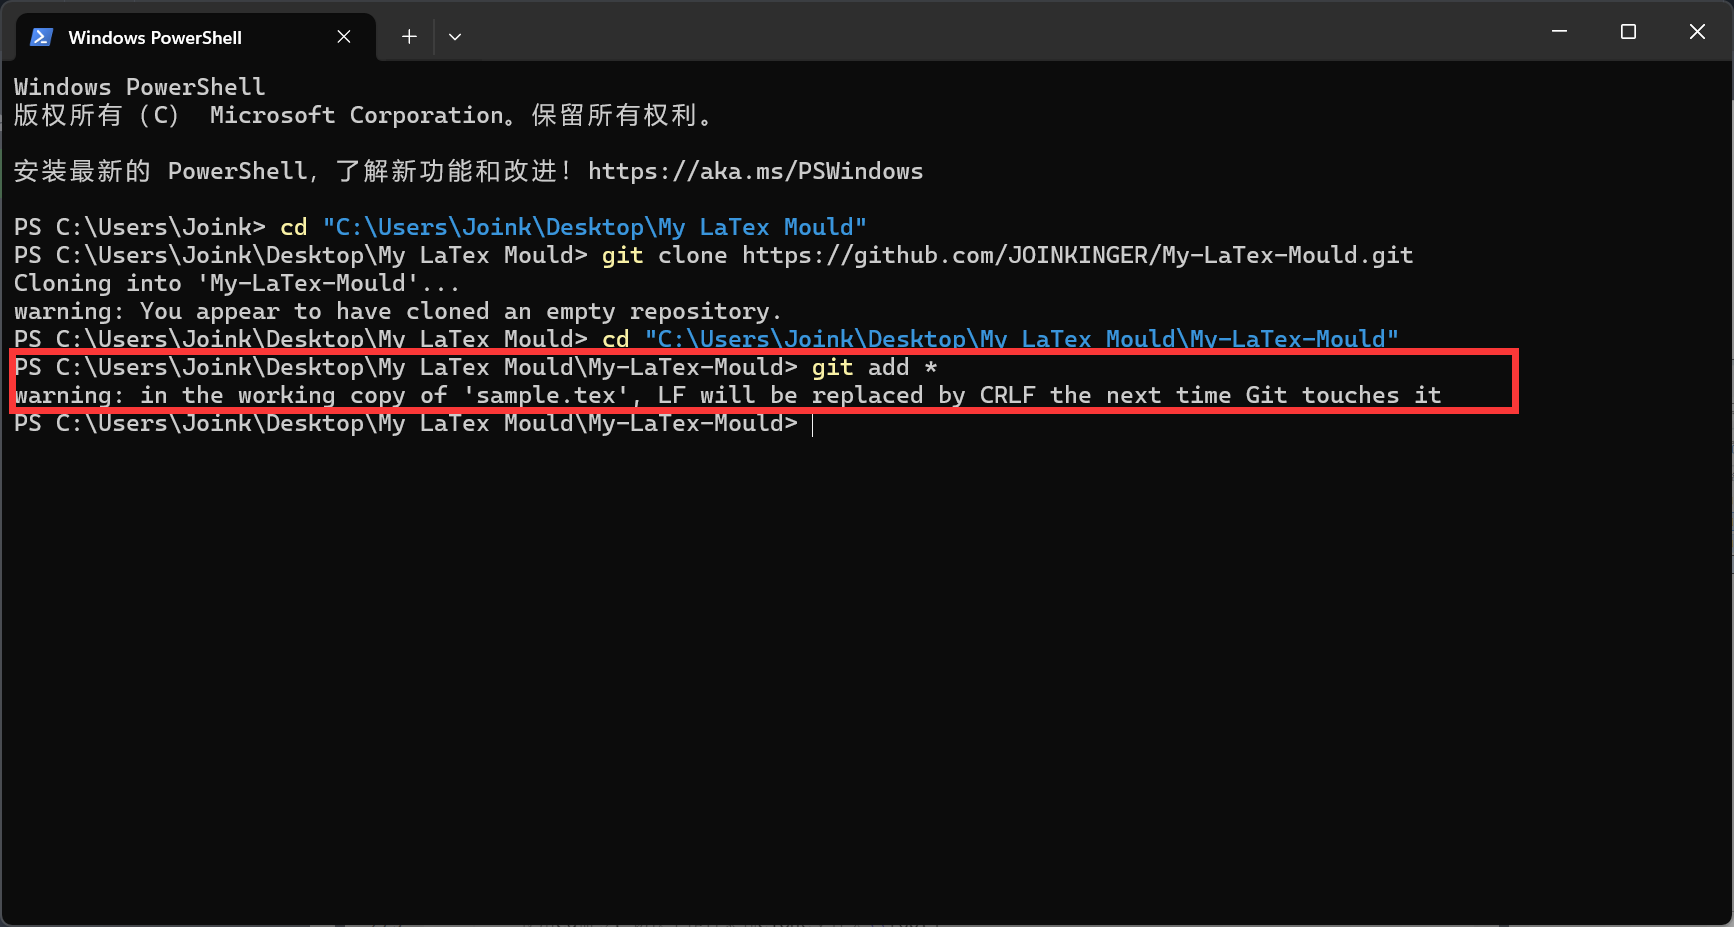
\includegraphics[scale=0.25]{pictures/git/17_3.png}\\
        \textcolor{red}{注:*表示上传所有文件}
        
        \item \textcolor{blue}{git commit命令}\\
        使用git commit命令,将暂存区的文件上传到本地git仓库中\\[6pt]
        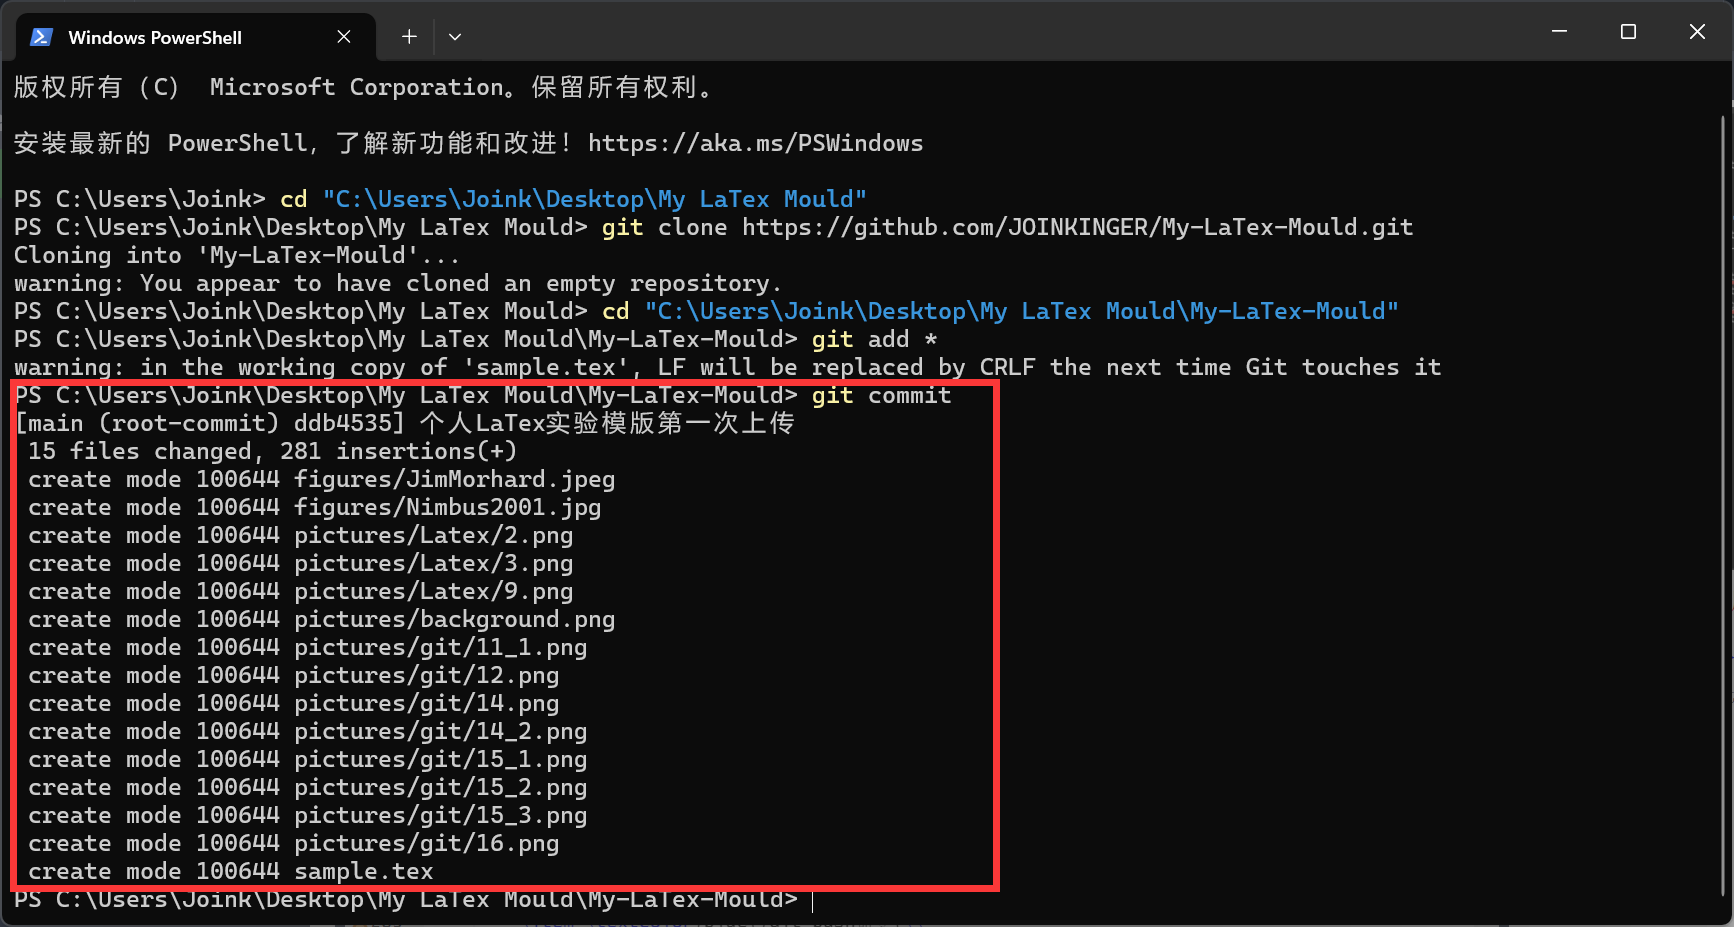
\includegraphics[scale=0.25]{pictures/git/18_1.png}\\
        此时进入vim编译器中\\
        按I进入INSERT(编辑)模式,输入提交日志\\[6pt]
        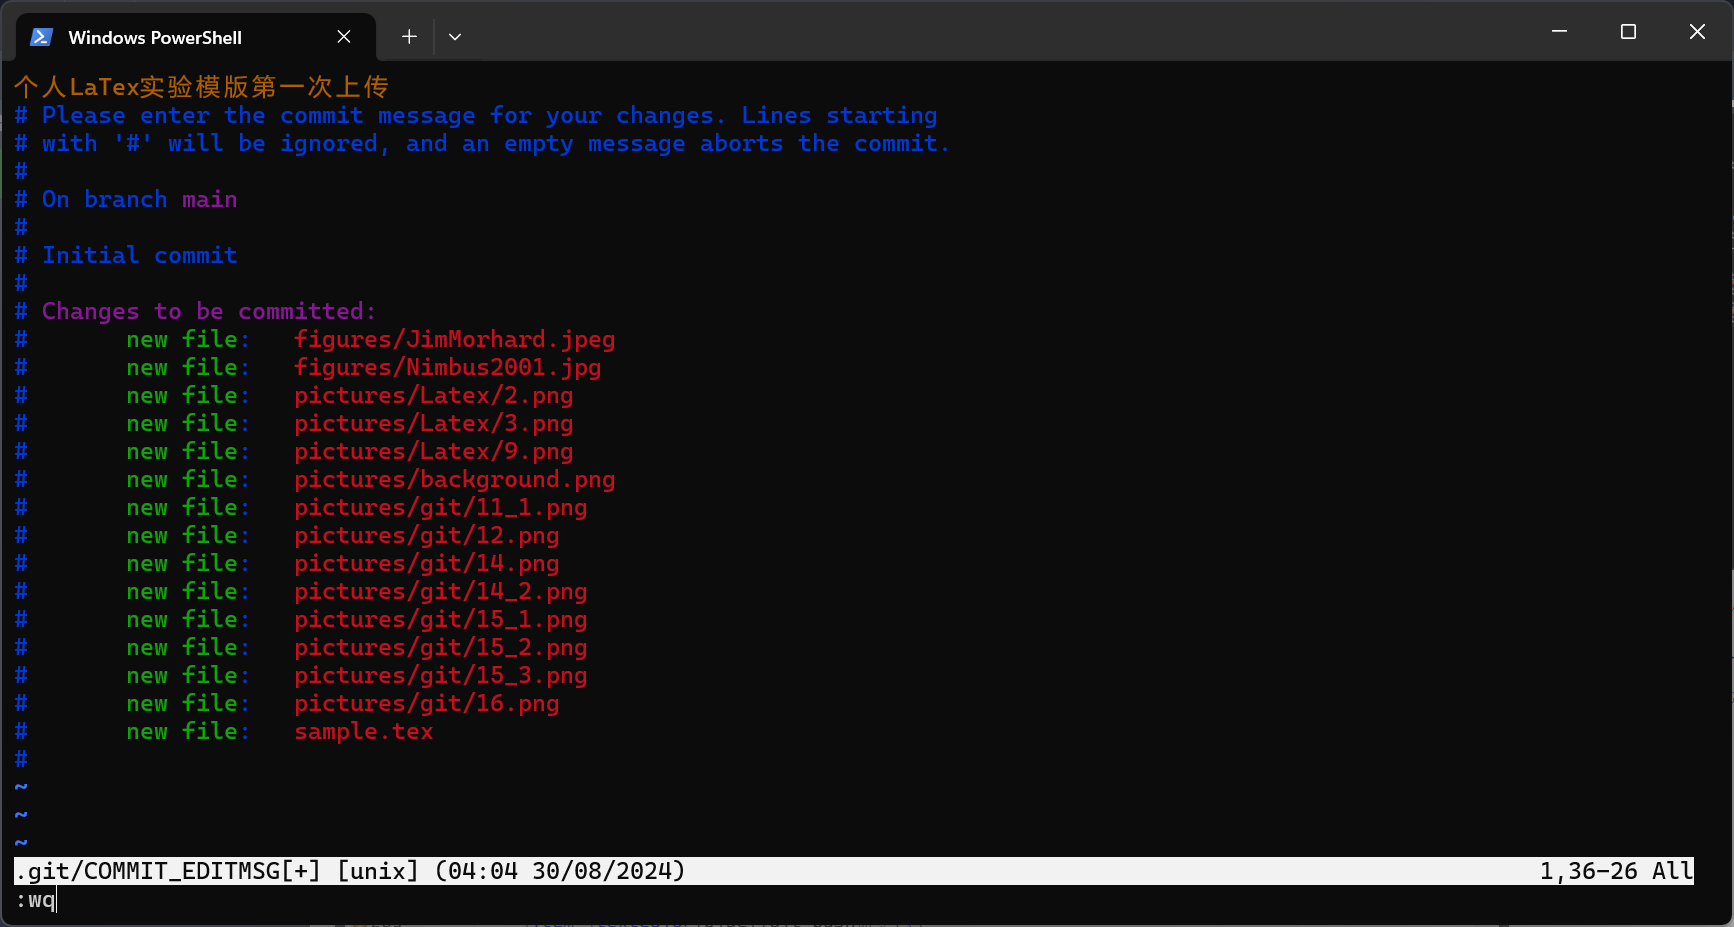
\includegraphics[scale=0.25]{pictures/git/18_3.png}\\
        输入完毕后按ESC退出INSERT模式,输入:wq保存并退出
        
        \item \textcolor{blue}{git push命令}\\
        使用git push命令,将上传到本地git仓库中的提交上传到github仓库中\\[6pt]
        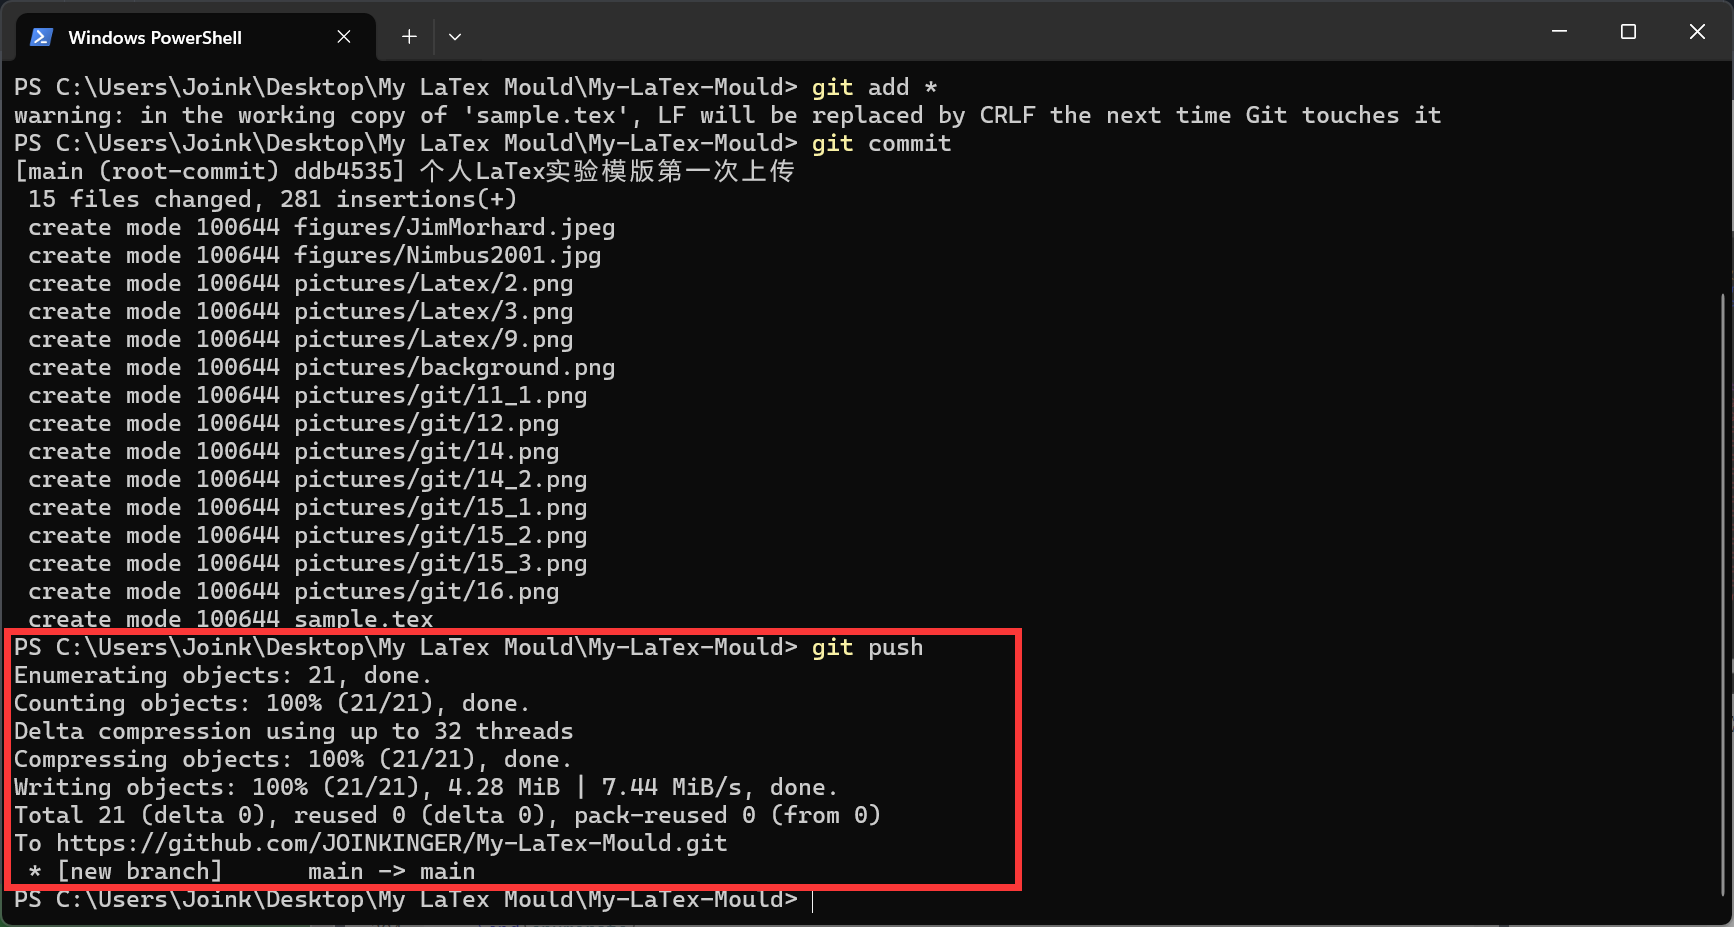
\includegraphics[scale=0.25]{pictures/git/19_1.png}\\
        刷新github网页,可以看到刚刚上传的提交\\[6pt]
        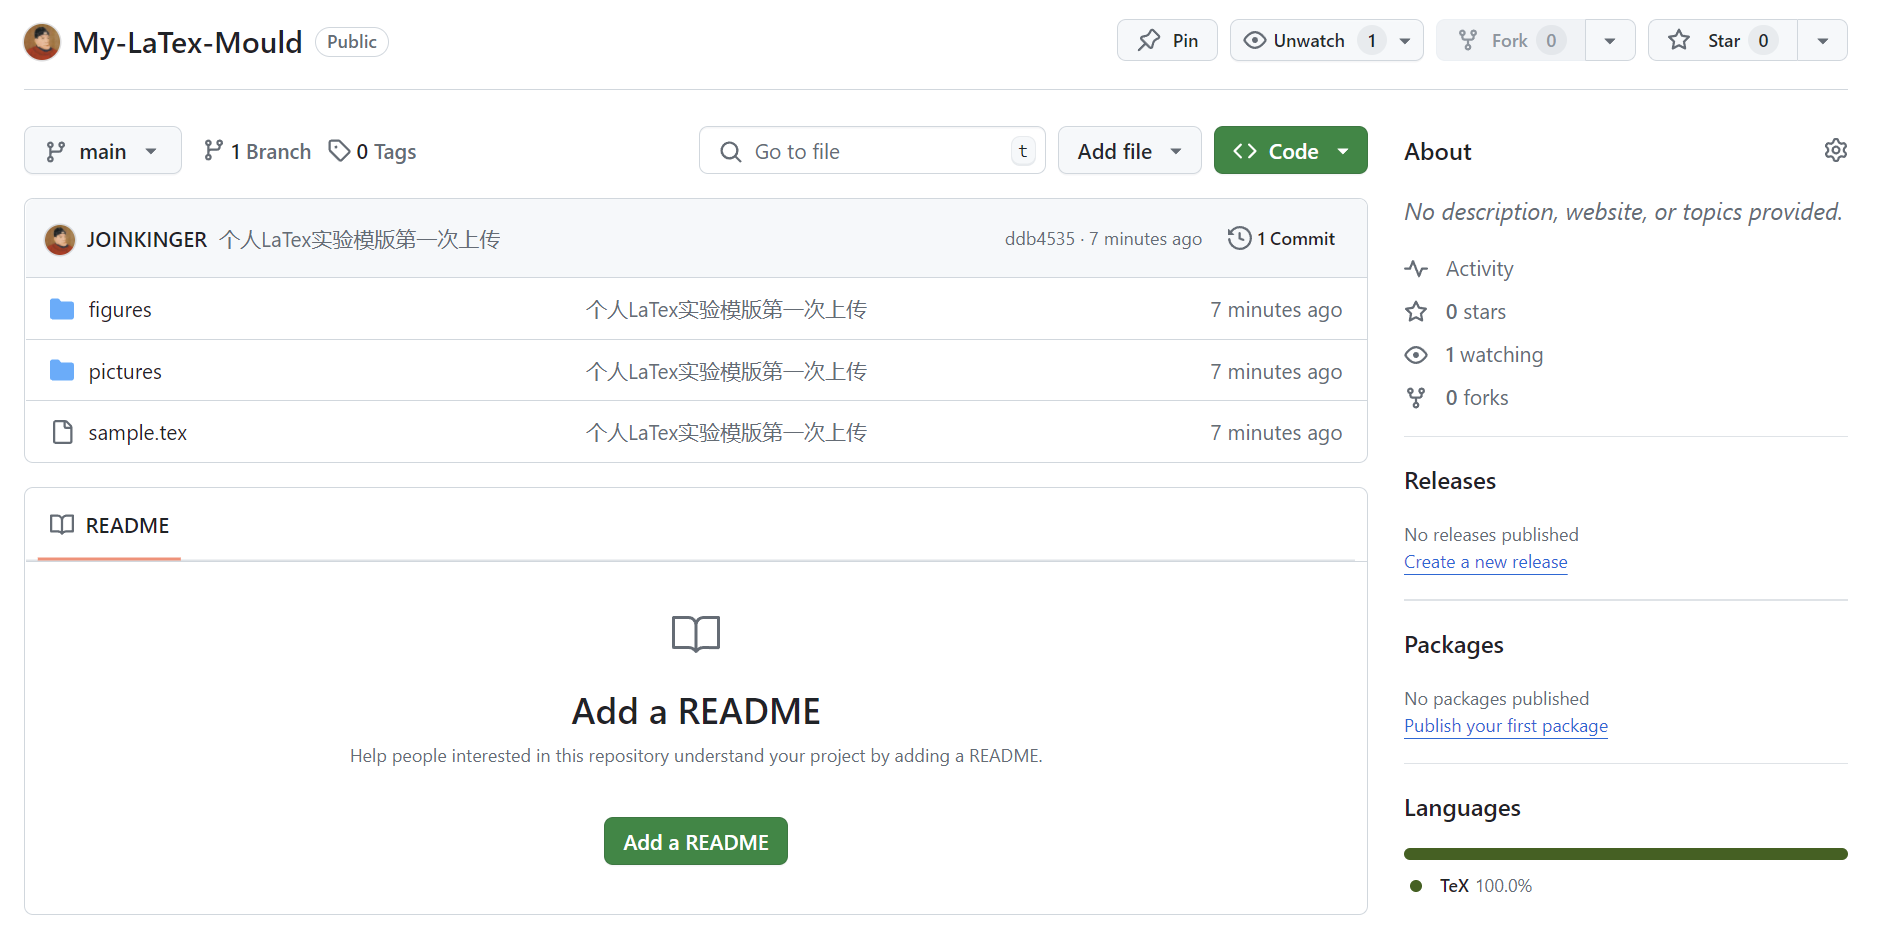
\includegraphics[scale=0.25]{pictures/git/19_2.png}    
        
        \item \textcolor{blue}{git log命令}\\
        由于git操作和LaTex文档编写同步进行,将此时的LaTex文件第二次上传\\[6pt]
        \includegraphics[scale=0.25]{}
        
        \item \textcolor{blue}{}\\
    \end{enumerate}

    \section{实验总结}
    本次实验中,扫帚被成功立起,证实了在不使用魔法的情况下,基本物理定律在霍格沃茨仍然适用。
\end{document}